\section{Consortium as a whole}
%Propongo: hacer mapa de Europa localizando los members of the committee. Coger información de los stakeholders del D1 y explicar porque somos un buen equipo. 
The consortium in charge of developing the DEOS-UD project has been chosen accurately in order to assure the capability of developing the project properly.

The consortium is made up of 8 different partners distributed in 5 different countries as shown in Figure \ref{consortium}. The members of the consortium have a wide knowhow and expertise in the areas covered in the project:

\begin{itemize}
\item Research in space technology and innovative design: HIRO, Aribus Defence and Space, ICUBE-SERTIT.
\item Development, testing and validation of space systems: Airbus Defence and Space, Deimos Space, Thales Alenia Space.
\item Data application for urban development: ReSAC and VITO.
\end{itemize} 

Apart from the technical aspects of the project, there are also partners with high expertise in project management, intellectual property management, data protection and exploitation and business plan specialized in space systems and applications (HIRO and BHO Legal Rechtsanwälte).

The consortium is well-structured and balanced among different experimented organisation and people who will bring the best expertise for each of the project objectives development.

During the project each partner has a well-defined role to play and no overlapping of activities will happen. However, the consortium is strong and would be capable of achieving the project expectations in case one partner leaves the project because another partner might perfectly be in charge of the remaining tasks. The consortium is characterised by a major presence of industrial organisation (3 large and 1 SME) guarantees the succes of the DEOS-UD project development and the presence of research specialized organization (ICUBE-SERTIT, ReSAC, HIRO and VITO) assure the innovation needed will be achieved. The balance between different organisations with different complementary knowledge areas is the most suitable for the development of the purpose of the project.

\begin{figure}[H]
\centering
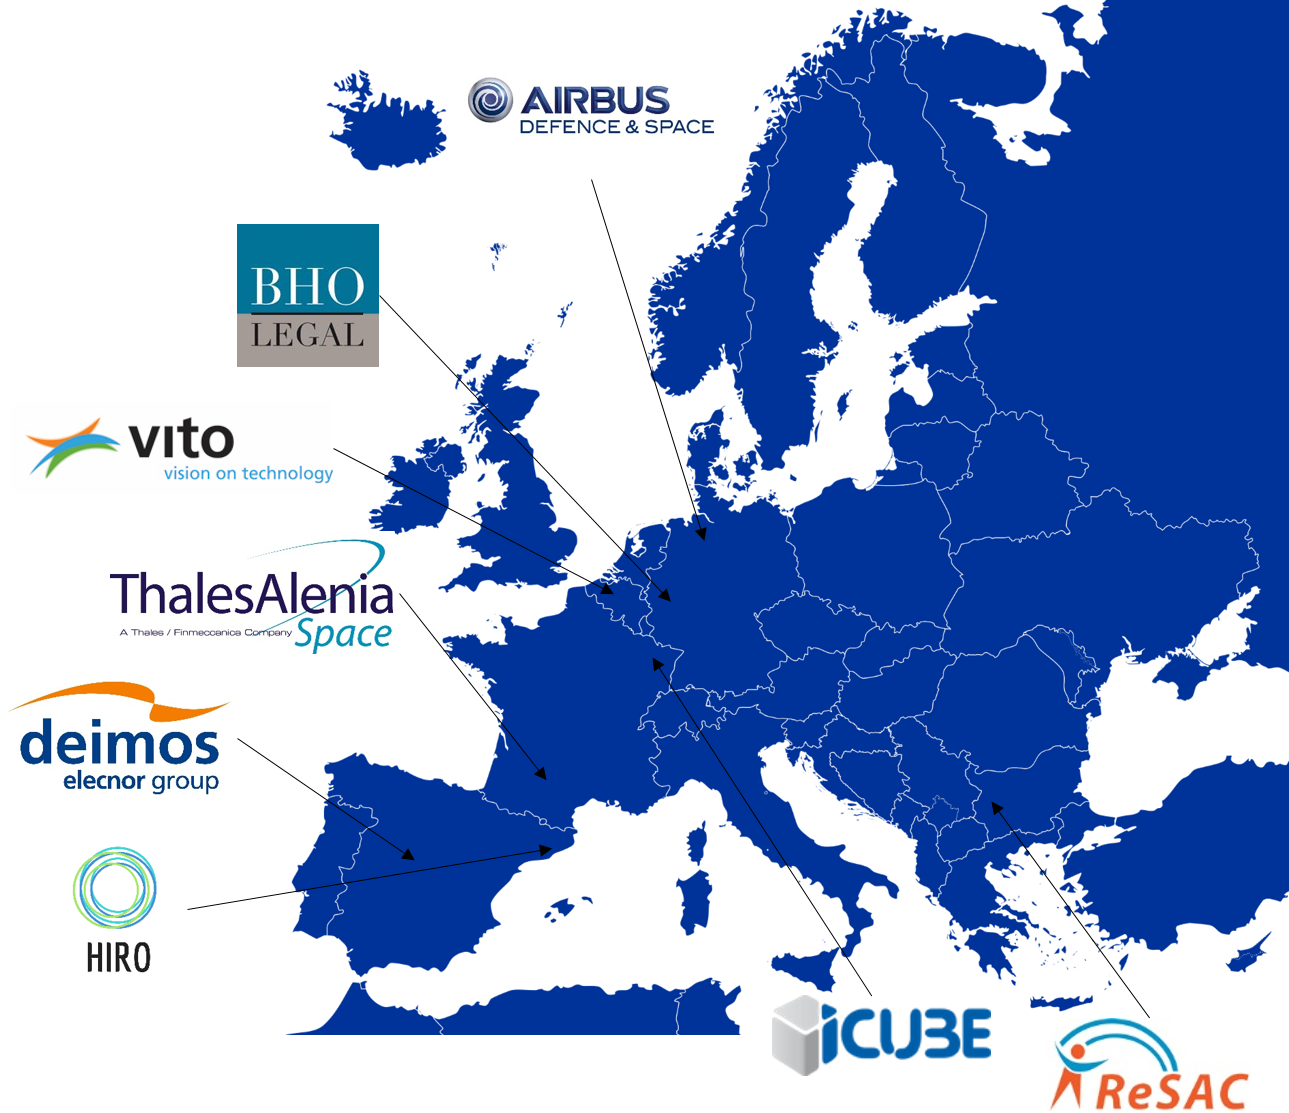
\includegraphics[width=\textwidth]{images/consortium.png} 
\caption{Consortium partners.}
\label{consortium}
\end{figure}